\chapter{Hardware}
\label{cha:hardware}
\section{Pepper}
\label{sec:pepper}
Pepper is a child sized humanoid social robot manufactured by SoftBank Robotics Group Corp.,
which can fulfill a wide range of purposes in different fields. Pepper is for example in
retail a lot to inform customers about special offers or articles in general. But it can also
be used as a receptionist in hotels or for entertainment in nursing homes.

\begin{figure}
\centering
\begin{subfigure}{.5\textwidth}
  \centering
  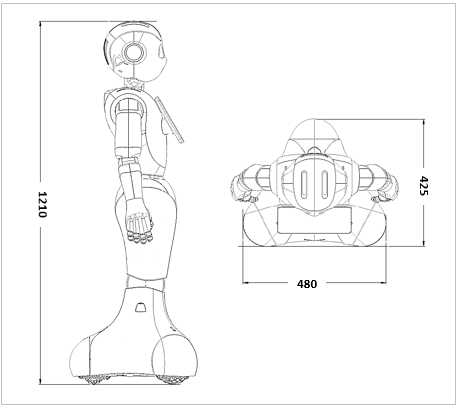
\includegraphics[width=\linewidth]{Pepper2.png}
  \caption{Measures without arms \cite{Pepper2018}}
\end{subfigure}%
\begin{subfigure}{.5\textwidth}
  \centering
  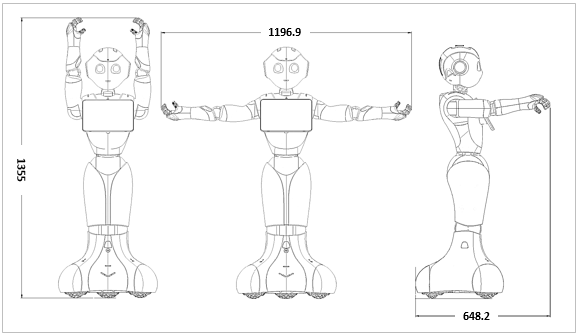
\includegraphics[width=\linewidth]{Pepper.png}
  \caption{Measures with arms \cite{Pepper2018}}
\end{subfigure}
\label{fig:pepper}
\end{figure}


It comes with the following sensors to perceive its surrounding:
\subsection*{Sensors}
\begin{description}
  \item [Inertial unit] Pepper is equipped with an Inertial unit, made of:
    \begin{itemize}
      \item a 3-axis gyroscope with an angular speed of ~500 °/s,
      \item a 3-axis accelerometer with an acceleration of ~2 g.
    \end{itemize}
  \item [Lasers] Pepper is equipped with 6 laser sensors which lets him evaluate its surrounding and the ground in front of it.
  \item [Infra-Red] Pepper is equipped with 2 infra-red sensors for obstacle detection
  \item [Sonars] Pepper is equipped with two ultrasonic sensors (or sonars) which allow it to estimate the distance to obstacles in its environment.
  \item [MRE] Peppers servo motors use MRE (Magnetic Rotary Encoders) using Hall-effect sensor technology.
  \item [Contact and tactile sensors] Pepper is equipped with different buttons and tactile sensors:
    \begin{itemize}
      \item Power button
      \item Emergency switch
      \item 3 tactile sensors on the head
      \item One tactile sensor on the back of every hand
      \item 3 bumpers on the base
    \end{itemize}
  \item [Video \& depth sensors] Pepper is equipped with a depth camera in the eyes and one camera in the mouth and another one in its head.
  \item [Microphones] Pepper is equipped with 4 microphones on its head to allow echo location
\end{description}

\begin{figure}
  \centering
  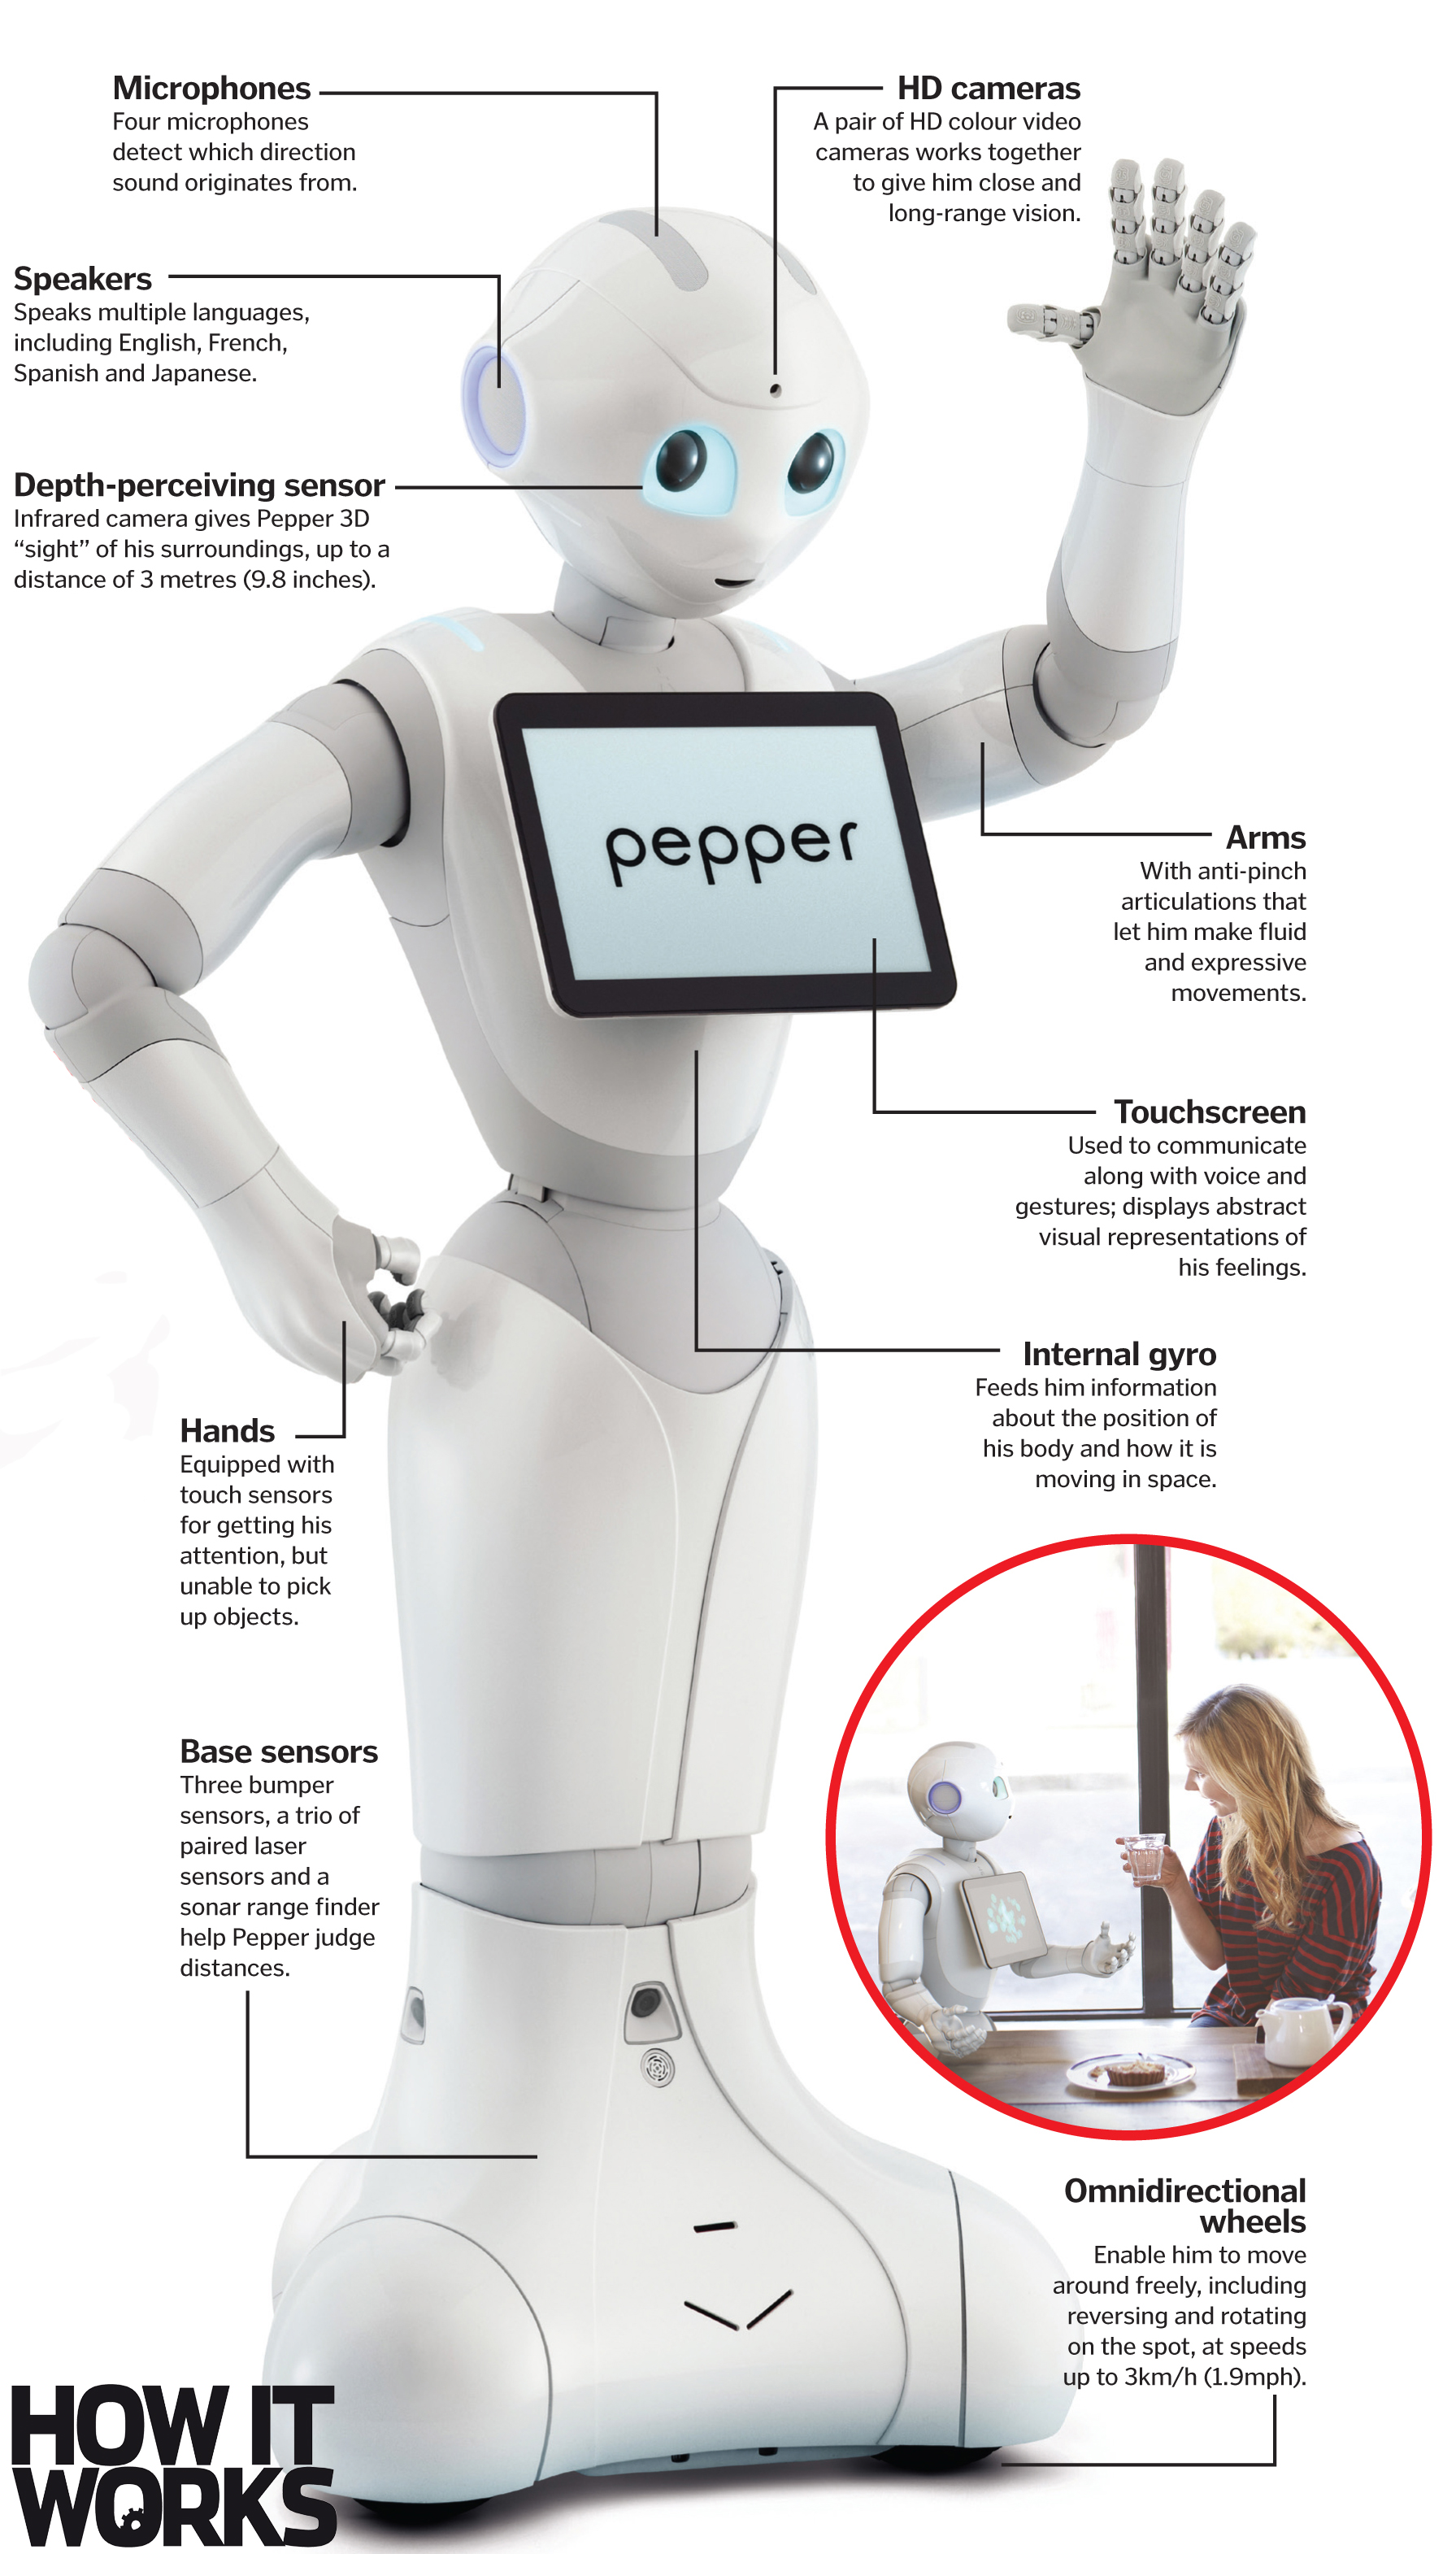
\includegraphics[width=.75\textwidth]{PepperOverview.jpg}
  \caption{Overview for Peppers sensors and actuators. \cite{pepperOverview}}
  \label{fig:pepperOverview}
\end{figure}

\subsection*{Actuators}
To act on the data acquired through the sensors Pepper has the following actuators:
\begin{description}
  \item [Loudspeakers] To speak very naturally to humans Pepper has two loudspeakers in its ears
  \item [LEDs] To indicate different signals Pepper uses LEDs in its shoulder, ears and eyes.
  \item [Motors] Pepper is equipped with a bunch of motors to move itself and different parts of its body:
  \begin{description}
    \item [Head] Pepper has motors for head yaw	and head pitch to move the field of view.
    \item [Arms] Pepper has motors for shoulder pitch, shoulder roll, elbow yaw and elbow roll to move the arms for gestures
    \item [Hands] Pepper has motors for wrist yaw	and grasping for gestures
    \item [Legs] Pepper has motors hip roll, hip pitch and knee pitch for leaning for- and backward.
    \item [Base] Pepper has motors for the 3 omnidirectional wheels on the base to drive around.
  \end{description}
\end{description}

\subsection*{Tablet}
Besides all the listed sensors and actuators Pepper is also equipped with a tablet, which gives the robot another feature for communication with humans. The tablet can be seen as an extra hybrid sensing and acting system, because it has sensing capabilities with the built-in camera and the touchscreen, but it also provides an actuator with the screen.

\subsection*{Internals}
To complete the robotic system a central processing unit and power supply is needed.
Pepper therefore is equipped with a Atom E3845 Quad core and 4 GB DDR3 RAM as well as a Lithium-ion battery with a capacity of 30 Ah, which lets Pepper operate for a whole workday without the need to recharge.
To communicate with other electronic devices Pepper is also equipped with a WiFi-chip which provides the IEEE 802.11 a/b/g/n standard and a Bluetooth-chip of Version 4.0.

To see the detailed description and illustrations of Pepper we forward the interested reader to \cite{Pepper2018}

